\begin{center}
\begin{figure}[!ht]
\centering
\subfloat[Unsorted]{\includegraphics[width=.5\textwidth]{../images/zipfRankedFull.png}}
\subfloat[Sorted]{\includegraphics[width=.5\textwidth]{../images/zipfAllSorted.png}}
\caption{Frequency Vs. Rank in full data, target, and other classes}
\label{fig:largecompare}
\end{figure}
\end{center}


\begin{tabular}{lcc}
\hline
& Mean & STD \\
\hline
svm & .9600 & 2.3406e-16\\
svm pca & 0.9400 & 2.3406e-16\\
ridge & 0.9400 & 2.3406e-16\\
lasso pca & 0.9460 & 0 \\
naivebayes smooth rand & 0.6826 & 0.0226\\
naivebayes smooth pca small & 0.9060 & 0\\
naivebayes smooth pca & 0.7680 & 1.1703e-16\\
lasso & 0.9380 & 0\\
naivebayes smooth & 0.6260 & 1.1703e-16
\end{tabular}

\begin{center}
\begin{figure}[!ht]
\centering
\subfloat[Accuracy]{\includegraphics[width=.7\textwidth]{../images/c3.png}}
\subfloat[Legend]{\includegraphics[width=.3\textwidth]{../images/legend.png}}
\caption{Accuracy vs Size of subsampled training data used.}
\label{fig:largecompare}
\end{figure}
\end{center}

\begin{center}
\begin{figure}[!ht]
\centering
\includegraphics[width=.7\textwidth]{../images/c3time.png}
\caption{Time vs Size of subsampled training data used.}
\label{fig:largecompare}
\end{figure}
\end{center}

\begin{center}
\begin{figure}[!ht]
\centering
\includegraphics[width=.7\textwidth]{../images/c3zoombig.png}
\caption{Accuracy vs Size of subsampled training data used.}
\label{fig:largecomparekleg}
\end{figure}
\end{center}

\begin{center}
\begin{figure}[!ht]
\centering
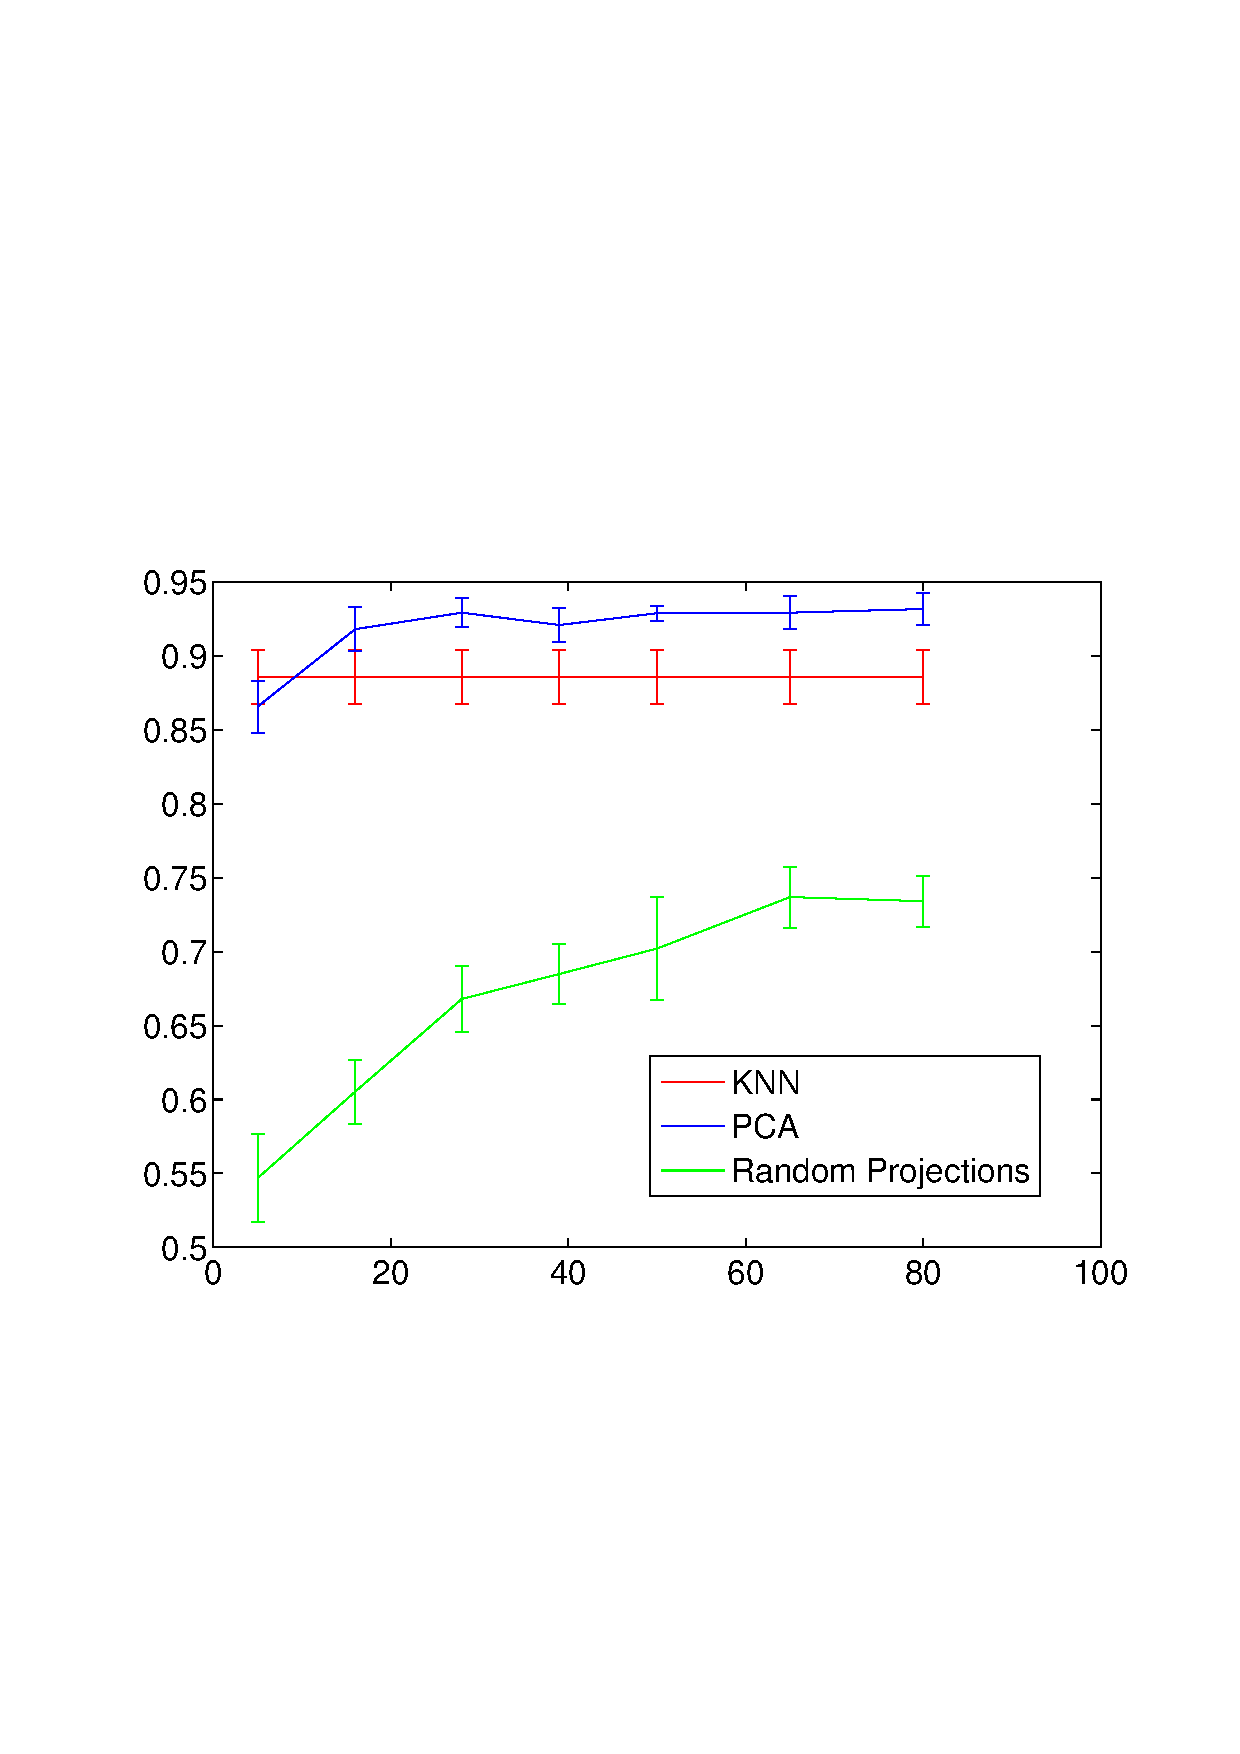
\includegraphics[width=.7\textwidth]{../images/knnVpcaVrproj.png}
\caption{Accuracy vs Dimensionality reduction size training with KNN.}
\label{fig:knn}
\end{figure}
\end{center}

\begin{center}
\begin{figure}[!ht]
\centering
\includegraphics[width=.7\textwidth]{../images/precisionrecallExpansion.png}
\caption{Precision and Recall vs. Number of features selected using LASSO.}
\label{fig:prec recall}
\end{figure}
\end{center}

\begin{center}
\begin{figure}[!ht]
\centering
\includegraphics[width=.7\textwidth]{../images/precisionrecallExpansion.png}
\caption{Precision and Recall vs. Number of features selected using LASSO.}
\label{fig:prec recall}
\end{figure}
\end{center}

\begin{tabular}{cccccccccccc}
\hline
Mean&Mean STD&Native Mean&Native STD&Mean Benefit&Benefit STD
\\
\hline
0.9272&0.0099&0.9256&0.0123&-0.0016&0.0069
\end{tabular}


\begin{tabular}{cccccccccccc}
\hline
Precision Mean&Precision STD&Recall Mean&Recall STD
\\
\hline
.7570&0.2913&0.9456&0.1662
\end{tabular}


\begin{tabular}{cccccccccccc}
\hline
Mean Redundant At&Redundant At STD\\
\hline
72.5000&9.6982
\end{tabular}
